\documentclass{article}
\usepackage{tikz}
\usepackage{amsmath}
\usepackage{bm}  % put in preamble
\usepackage{empheq}
\usetikzlibrary{arrows.meta,calc,decorations.pathreplacing}

\title{Physics of vehicle dynamics}
\author{v4m3rrr}
\date{\today}

\begin{document}
	\maketitle
	\tableofcontents
	\newpage
	\section{Weight transfer}
	Weight transfer is a fundamental concept in vehicle dynamics that describes how the normal loads on the tires change when a vehicle accelerates, brakes, or turns. Although the total weight of the vehicle remains constant, the distribution of this weight among the tires shifts because of the inertia of the mass acting through the center of gravity.
	
	During cornering, the lateral acceleration produces a moment about the vehicle’s roll axis, causing additional load to be transferred from the inside wheels to the outside wheels. This lateral weight transfer affects the available tire grip on each side, influencing handling balance, cornering performance, and ultimately vehicle stability.
	\begin{figure}[h]
		\centering
		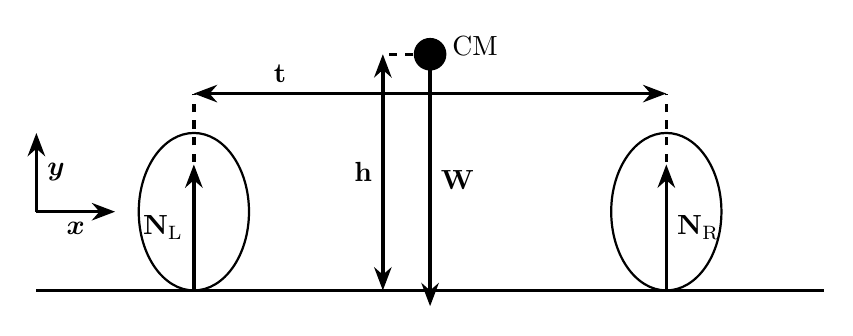
\begin{tikzpicture}[scale=2.0, >=Stealth, every node/.style={font=\normalsize}]
			
			% parameters
			\def\wheelsep{3.0}     % distance between wheel centers
			\def\wheeldia{0.9}     % wheel diameter
			\def\bodyh{1.0}        % rear body height above axle
			\def\axlepos{0.0}      % y position of axle/ground
			\def\cgx{0.0}          % horizontal offset of CG from midline (+ forward)
			\def\cgz{1.0}          % vertical position of CG above ground
			\def\wheelbigradius{0.5}
			
			% ground line
			\draw[thick] (-1,0) -- (\wheelsep+1,0);
			
			% wheel centers (two rear wheels)
			\coordinate (WL) at (0,0.5);
			\coordinate (WR) at (\wheelsep,0.5);
			
			% draw wheels
			%\draw[thick] (WL) circle[radius=0.5];
			%\draw[thick] (WR) circle[radius=0.5];
			\draw[thick] (WL) ellipse (0.35 and 0.5); 
			\draw[thick] (WR) ellipse (0.35 and 0.5); 
			
			
			% center of gravity (cg)
			\coordinate (CG) at ($(WL)!0.5!(WR) + (\cgx,\cgz)$);
			\draw[fill=black] (CG) circle (0.1);
			\node[right] at ($(CG)+(0.08,0.05)$) {CM};
			
			% weight
			\draw[very thick, ->] (CG) -- ++(0,-1.6) 
			node[midway,right] {$\mathbf{W}$};
			
			% normals
			\draw[very thick, ->] ($(WL)+(0,-\wheelbigradius)$) -- ++(0,0.8) 
			node[midway,left] {$\mathbf{N}_\text{L}$};
			\draw[very thick, ->] ($(WR)+(0,-\wheelbigradius)$) -- ++(0,0.8) 
			node[midway,right] {$\mathbf{N}_\text{R}$};
			
			% elipse
			\draw[very thick, <->] (0,2.5*\wheelbigradius) node[above right,xshift=25] {$\mathbf{t}$} -- (\wheelsep,2.5*\wheelbigradius) ;
			\draw[very thick, dashed, -] ($(WL)$) -- (0,2.5*\wheelbigradius);
			\draw[very thick, dashed, -] ($(WR)$) -- (\wheelsep,2.5*\wheelbigradius);
			
			\draw[very thick,dashed, -] (CG) -- ++(-0.3,0);
			\draw[very thick, <->] ($(CG)+(-0.3,0)$) -- (\wheelsep/2-0.3,0)
			node[midway, left] {$\mathbf{h}$};
			
			\draw[very thick, ->] ($(WL)+(-1,0)$) -- ++(0.5,0) 
			node[midway,below] {$\bm{x}$};
			\draw[very thick, ->] ($(WL)+(-1,0)$) -- ++(0,0.5) 
			node[midway,right] {$\bm{y}$};
		\end{tikzpicture}
		\caption{Free body diagram of a car when stationary (viewed from behind).}
		\label{fig:stationary}
	\end{figure}
	
	\begin{figure}[h]
		\centering
		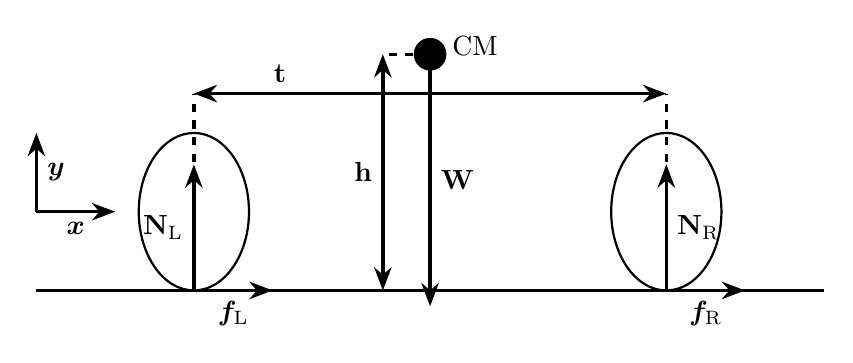
\begin{tikzpicture}[scale=2.0, >=Stealth, every node/.style={font=\normalsize}]
			
			% parameters
			\def\wheelsep{3.0}     % distance between wheel centers
			\def\wheeldia{0.9}     % wheel diameter
			\def\bodyh{1.0}        % rear body height above axle
			\def\axlepos{0.0}      % y position of axle/ground
			\def\cgx{0.0}          % horizontal offset of CG from midline (+ forward)
			\def\cgz{1.0}          % vertical position of CG above ground
			\def\wheelbigradius{0.5}
			
			% ground line
			\draw[thick] (-1,0) -- (\wheelsep+1,0);
			
			% wheel centers (two rear wheels)
			\coordinate (WL) at (0,0.5);
			\coordinate (WR) at (\wheelsep,0.5);
			
			% draw wheels
			%\draw[thick] (WL) circle[radius=0.5];
			%\draw[thick] (WR) circle[radius=0.5];
			\draw[thick] (WL) ellipse (0.35 and 0.5); 
			\draw[thick] (WR) ellipse (0.35 and 0.5); 
			
			
			% center of gravity (cg)
			\coordinate (CG) at ($(WL)!0.5!(WR) + (\cgx,\cgz)$);
			\draw[fill=black] (CG) circle (0.1);
			\node[right] at ($(CG)+(0.08,0.05)$) {CM};
			
			% weight
			\draw[very thick, ->] (CG) -- ++(0,-1.6) 
			node[midway,right] {$\mathbf{W}$};
			
			% normals
			\draw[very thick, ->] ($(WL)+(0,-\wheelbigradius)$) -- ++(0,0.8) 
			node[midway,left] {$\mathbf{N}_\text{L}$};
			\draw[very thick, ->] ($(WR)+(0,-\wheelbigradius)$) -- ++(0,0.8) 
			node[midway,right] {$\mathbf{N}_\text{R}$};
			
			% elipse
			\draw[very thick, <->] (0,2.5*\wheelbigradius) node[above right,xshift=25] {$\mathbf{t}$} -- (\wheelsep,2.5*\wheelbigradius) ;
			\draw[very thick, dashed, -] ($(WL)$) -- (0,2.5*\wheelbigradius);
			\draw[very thick, dashed, -] ($(WR)$) -- (\wheelsep,2.5*\wheelbigradius);
			
			\draw[very thick,dashed, -] (CG) -- ++(-0.3,0);
			\draw[very thick, <->] ($(CG)+(-0.3,0)$) -- (\wheelsep/2-0.3,0)
			node[midway, left] {$\mathbf{h}$};
			
			\draw[very thick, ->] ($(WL)+(0,-\wheelbigradius)$) -- ++(0.5,0) 
			node[midway,below] {$\bm{f}_\text{L}$};
			\draw[very thick, ->] ($(WR)+(0,-\wheelbigradius)$) -- ++(0.5,0) 
			node[midway,below] {$\bm{f}_\text{R}$};
			
			\draw[very thick, ->] ($(WL)+(-1,0)$) -- ++(0.5,0) 
			node[midway,below] {$\bm{x}$};
			\draw[very thick, ->] ($(WL)+(-1,0)$) -- ++(0,0.5) 
			node[midway,right] {$\bm{y}$};
		\end{tikzpicture}
		\caption{Free body diagram of a car when turning to right (viewed from behind).}
		\label{fig:turning}
	\end{figure}
	Since the body does not move in the vertical ($y$) direction, the vertical force balance is
	\begin{align}
	W=N_L+N_R
	\label{eq:y_equal}
	\end{align}
	where $W = mg$ is the total weight and $N_L$, $N_R$ are the left and right normal forces.
	
	When the car moves along a curved path, a centripetal force is required:
	\begin{align}
		F_c=f_L+f_R
		\label{eq:centrifugal}
	\end{align}
	where $f_L$ and $f_R$ are the lateral tire forces. The magnitude of this force is
	\begin{align}
		F_c = \frac{mv^2}{r} = ma_l
	\end{align}
	with $a_l$ the lateral acceleration.
	
	Taking moments about the center of mass, the torque balance is
	\begin{align}
		\tau_{CM}=Wr_W+f_Lh+f_Rh+N_R\frac{w}{2}-N_L\frac{w}{2}
	\end{align}
	Since the weight acts through the center of mass ($r_W=0$) and assuming the vehicle does not tip ($\tau_{CM}=0$), we obtain
	\begin{align}
		N_L = \frac{W}{2} + \frac{F_c h}{w}
	\end{align}
	Substituting $F_c = ma_l$ and $W=mg$ gives
	\begin{align}
		N_L = \frac{W}{2} + W \frac{a_l}{g}\frac{h}{w}
	\end{align}
	Defining the load transfer as
	\begin{align}
		\Delta W = W \frac{a_l}{g}\frac{h}{w}
	\end{align}
	the left and right wheel loads during a right-hand turn become
	\begin{empheq}[box=\fbox]{equation}
		N_L = \frac{W}{2} + \Delta W, \quad 
		N_R = \frac{W}{2} - \Delta W
	\end{empheq}
	and by symmetry, for a left-hand turn
	\begin{empheq}[box=\fbox]{equation}
		N_L = \frac{W}{2} - \Delta W \quad
		N_R = \frac{W}{2} + \Delta W
	\end{empheq}
	
	\section{Tire Adhesion}  
	
	The force of tire adhesion can be expressed as:  
	\begin{align}  
		F \leq \mu N  
	\end{align}  
	
	where:  
	\begin{itemize}  
		\item $\mu$ is the coefficient of adhesion,  
		\item $N$ is the normal load (weight acting on the tire).  
	\end{itemize}  
	
	The right-hand side of the inequality represents the maximum tractive or braking force that can be transmitted without slip. If this limit is exceeded, the tire transitions from static to kinetic friction, which results in loss of grip.  
	
	In practice, the coefficient of adhesion $\mu$ is not constant. It depends on several factors, including:  
	\begin{itemize}  
		\item Tire deformation and tread design,  
		\item Temperature of both tire and road surface,  
		\item Weather conditions (dry, wet, icy, snowy),  
		\item Tire inflation pressure,  
		\item Road texture and surface contamination (dust, oil, gravel, etc.).  
	\end{itemize}  
	
	A well-designed tire ensures a smooth transition between static and kinetic friction so that grip is not lost suddenly, which is crucial for vehicle stability and safety.    
	
	% Optional TikZ diagram for illustration:
	\begin{figure}[h]
		\centering
		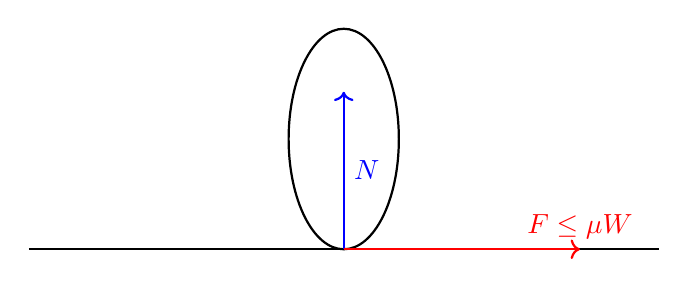
\begin{tikzpicture}[scale=2]
			% Road
			\draw[thick] (-2,0) -- (2,0);
			% Tire
			\draw[thick] (0,0.7) ellipse (0.35 and 0.7);
			% Normal force
			\draw[->, thick, blue] (0,0.0) -- (0,1) node[midway,right] {$N$};
			% Friction force
			\draw[->, thick, red] (0,0.0) -- (1.5,0.0) node[right,above] {$F \leq \mu W$};
		\end{tikzpicture}
		\caption{Forces acting on a tire in contact with the road.}
	\end{figure}
	
\end{document}
